\documentclass{standalone}
\makeatletter\AtBeginDocument{\@buildstepset{1,2,3,4,5}}\makeatother
\usepackage{hsbcommon}
\begin{document}
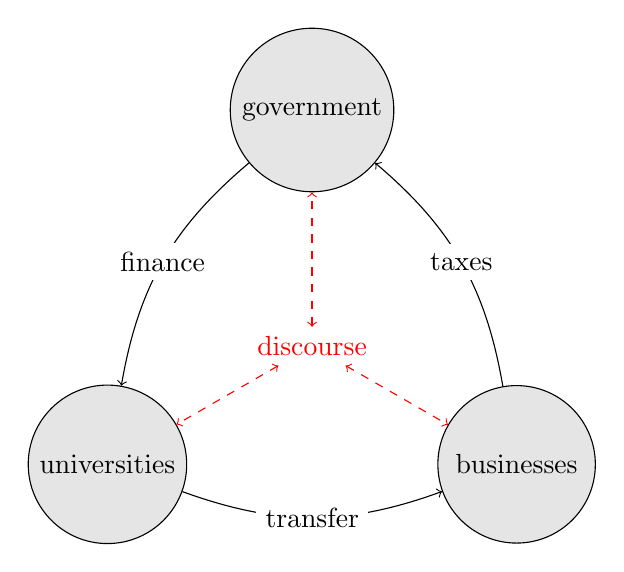
\begin{tikzpicture}[rotate=90]
    \foreach [count=\i] \myinst in {universities,businesses,government}
    {
        \node[draw,circle,minimum width=2cm,fill=gray!20] (N\i) at (\i*120:3) {\myinst};
    }
    \draw[->,bend right=20] (N1) to node[fill=white] {transfer}  (N2);
    \draw[->,bend right=20] (N2) to node[fill=white] {taxes}  (N3);
    \draw[->,bend right=20] (N3) to node[fill=white] {finance} (N1);


    \ifstep{1}{
        \begin{scope}[red]
            \node (D) at (0:0) {discourse};
            \foreach \i in {1,2,3} \draw[<->,dashed] (D) -- (N\i);
        \end{scope}
    }
    
\end{tikzpicture}
\end{document}